%%%%%%%%%%%%%%%%%%%%%%%%%%%%%%%%%%%%%%%%%%%%%%%%%%%%%%%%%%%%%%%%%%%%%%
%% LaTeX template for DTR Report: (look for \DTRPcs defined below)
%%
%% (c) 2023--2024 RTE
%% Developed by Grupo AIA
%%
%%%%%%%%%%%%%%%%%%%%%%%%%%%%%%%%%%%%%%%%%%%%%%%%%%%%%%%%%%%%%%%%%%%%%%
\documentclass[a4paper,11pt]{article}
\usepackage[utf8]{inputenc}
\usepackage[T1]{fontenc}
\usepackage[english]{babel}
\usepackage[tmargin=2cm, bmargin=1.5cm, lmargin=3cm, rmargin=3cm]{geometry}
\usepackage{hyperref}
\usepackage{graphicx}
\usepackage{xcolor}
\usepackage{dcolumn}  % for columns of dot-centered numbers in tables
\usepackage{booktabs}  % for better tables
\usepackage{bookmark}
\usepackage[cbgreek]{textgreek} % for the Dynawo "omega" font
\usepackage[mode=buildnew]{standalone}  % for TikZ figures
\usepackage{fancyhdr}
\usepackage{float}
\usepackage{environ}
\usepackage{expl3}
\usepackage{caption}
\usepackage{amstext}
\usepackage{ifthen}


%% More sensible colors for hyperref links:
\hypersetup{
    colorlinks = true, % color links instead of ugly boxes
    urlcolor   = blue, % color of external hyperlinks
    linkcolor  = dark-blue, % color of internal links
    citecolor  = red   % color of citations
}

% Short-hand column specifier for tables (uses dcolumn):
\newcolumntype{d}[1]{D{.}{.}{#1}}

% Fancy header
\fancyhf{}

%%%%%%%%%%%%%%%%%%%%%%%%%%%%%%%%%%%%%%%%%
%% From here on, our short-hand macros:
%%%%%%%%%%%%%%%%%%%%%%%%%%%%%%%%%%%%%%%%%
\newcommand{\code}[1]{\texttt{#1}}  % for code snippets
\newcommand{\Dynawo}{Dyna\textomega o} % but it doesn't show in bold
\newcommand{\PASS}{\textcolor{dark-green}{\textbf{PASS}}}
\newcommand{\FAIL}{\textcolor{red}{\textbf{FAIL}}}

%% Empty commands to use in PCS reports
%% We have to define them here first and then use renewcommands in the PCS reports
%% because the same reports are not always generated, so it is not possible
%% to uniquely identify which is the first one.
\newcommand{\DTRPcs}{} % DTR pcs definition
\newcommand{\DTRPcsLong}{}
\newcommand{\OCname}{}
\newcommand{\PCSName}{}

%% Our colors (for backgrounds and code listings):
\definecolor{light-gray}{gray}{0.9}
\definecolor{dark-gray}{gray}{0.4}
\definecolor{light-blue}{RGB}{64,64,255}
\definecolor{dark-blue}{RGB}{16,16,64}
\definecolor{dark-green}{RGB}{16,128,16}


%%%%%%%%%%%%%%%%%%%%%%%%%%%%%%%%%%%%%%%%%
%% The document starts here
%%%%%%%%%%%%%%%%%%%%%%%%%%%%%%%%%%%%%%%%%

\title{DGCV Report \\[1ex] \large {{verificationtype}}\\[1ex] \large for {{modeltype}}}
\author{RTE}
\date{
    \vspace{0.5cm}
    
\includegraphics[width=2cm]{TSO_logo}\\
    \vspace{0.5cm}
    \today
}
\lhead{Results from running DTR tests~\cite{DTRhome}, using \Dynawo~\cite{Dynawo}.}
\begin{document}

    \maketitle

    \newpage
    \thispagestyle{fancy}
    \tableofcontents

    \newpage
    \section{Summary}
    {{summary_description}}

    \begin{center}
        \begin{tabular}{ccccc}
            \toprule
            Producer & Pcs & Benchmark & Operating Condition & Overall Result \\
            \midrule
            \BLOCK{for row in summaryReport}
            {{row[0]}} & {{row[1]}} & {{row[2]}} & {{row[3]}} & {{row[4]}} \\
            \BLOCK{endfor}
            \bottomrule
        \end{tabular}
    \end{center}

    \BLOCK{for report in reports}
    \newpage
    {{report}}
    \BLOCK{endfor}

    \newpage
    \begin{thebibliography}{9}
      \bibitem{DTRhome} \textit{Documentation technique de référence en cours de
        validité.}  RTE. 2024. \textsc{url:}
        \url{https://www.services-rte.com/fr/decouvrez-nos-offres-de-service/raccorder-une-installation-de-production.html}.
      \bibitem{Dynawo} \textit{\Dynawo --- A hybrid C++/Modelica open source suite of
        simulation tools for power systems}. RTE. 2015--2024. \textsc{url:}
        \url{https://dynawo.github.io}.
    \end{thebibliography}

    \newpage
    \section*{Appendix: step-response characteristics}

    Illustration depicting the definition of the step-response characteristics,
    taken from IEC 61400-21-1 (Section 3, Terms and definitions).\\[1.5cm]
    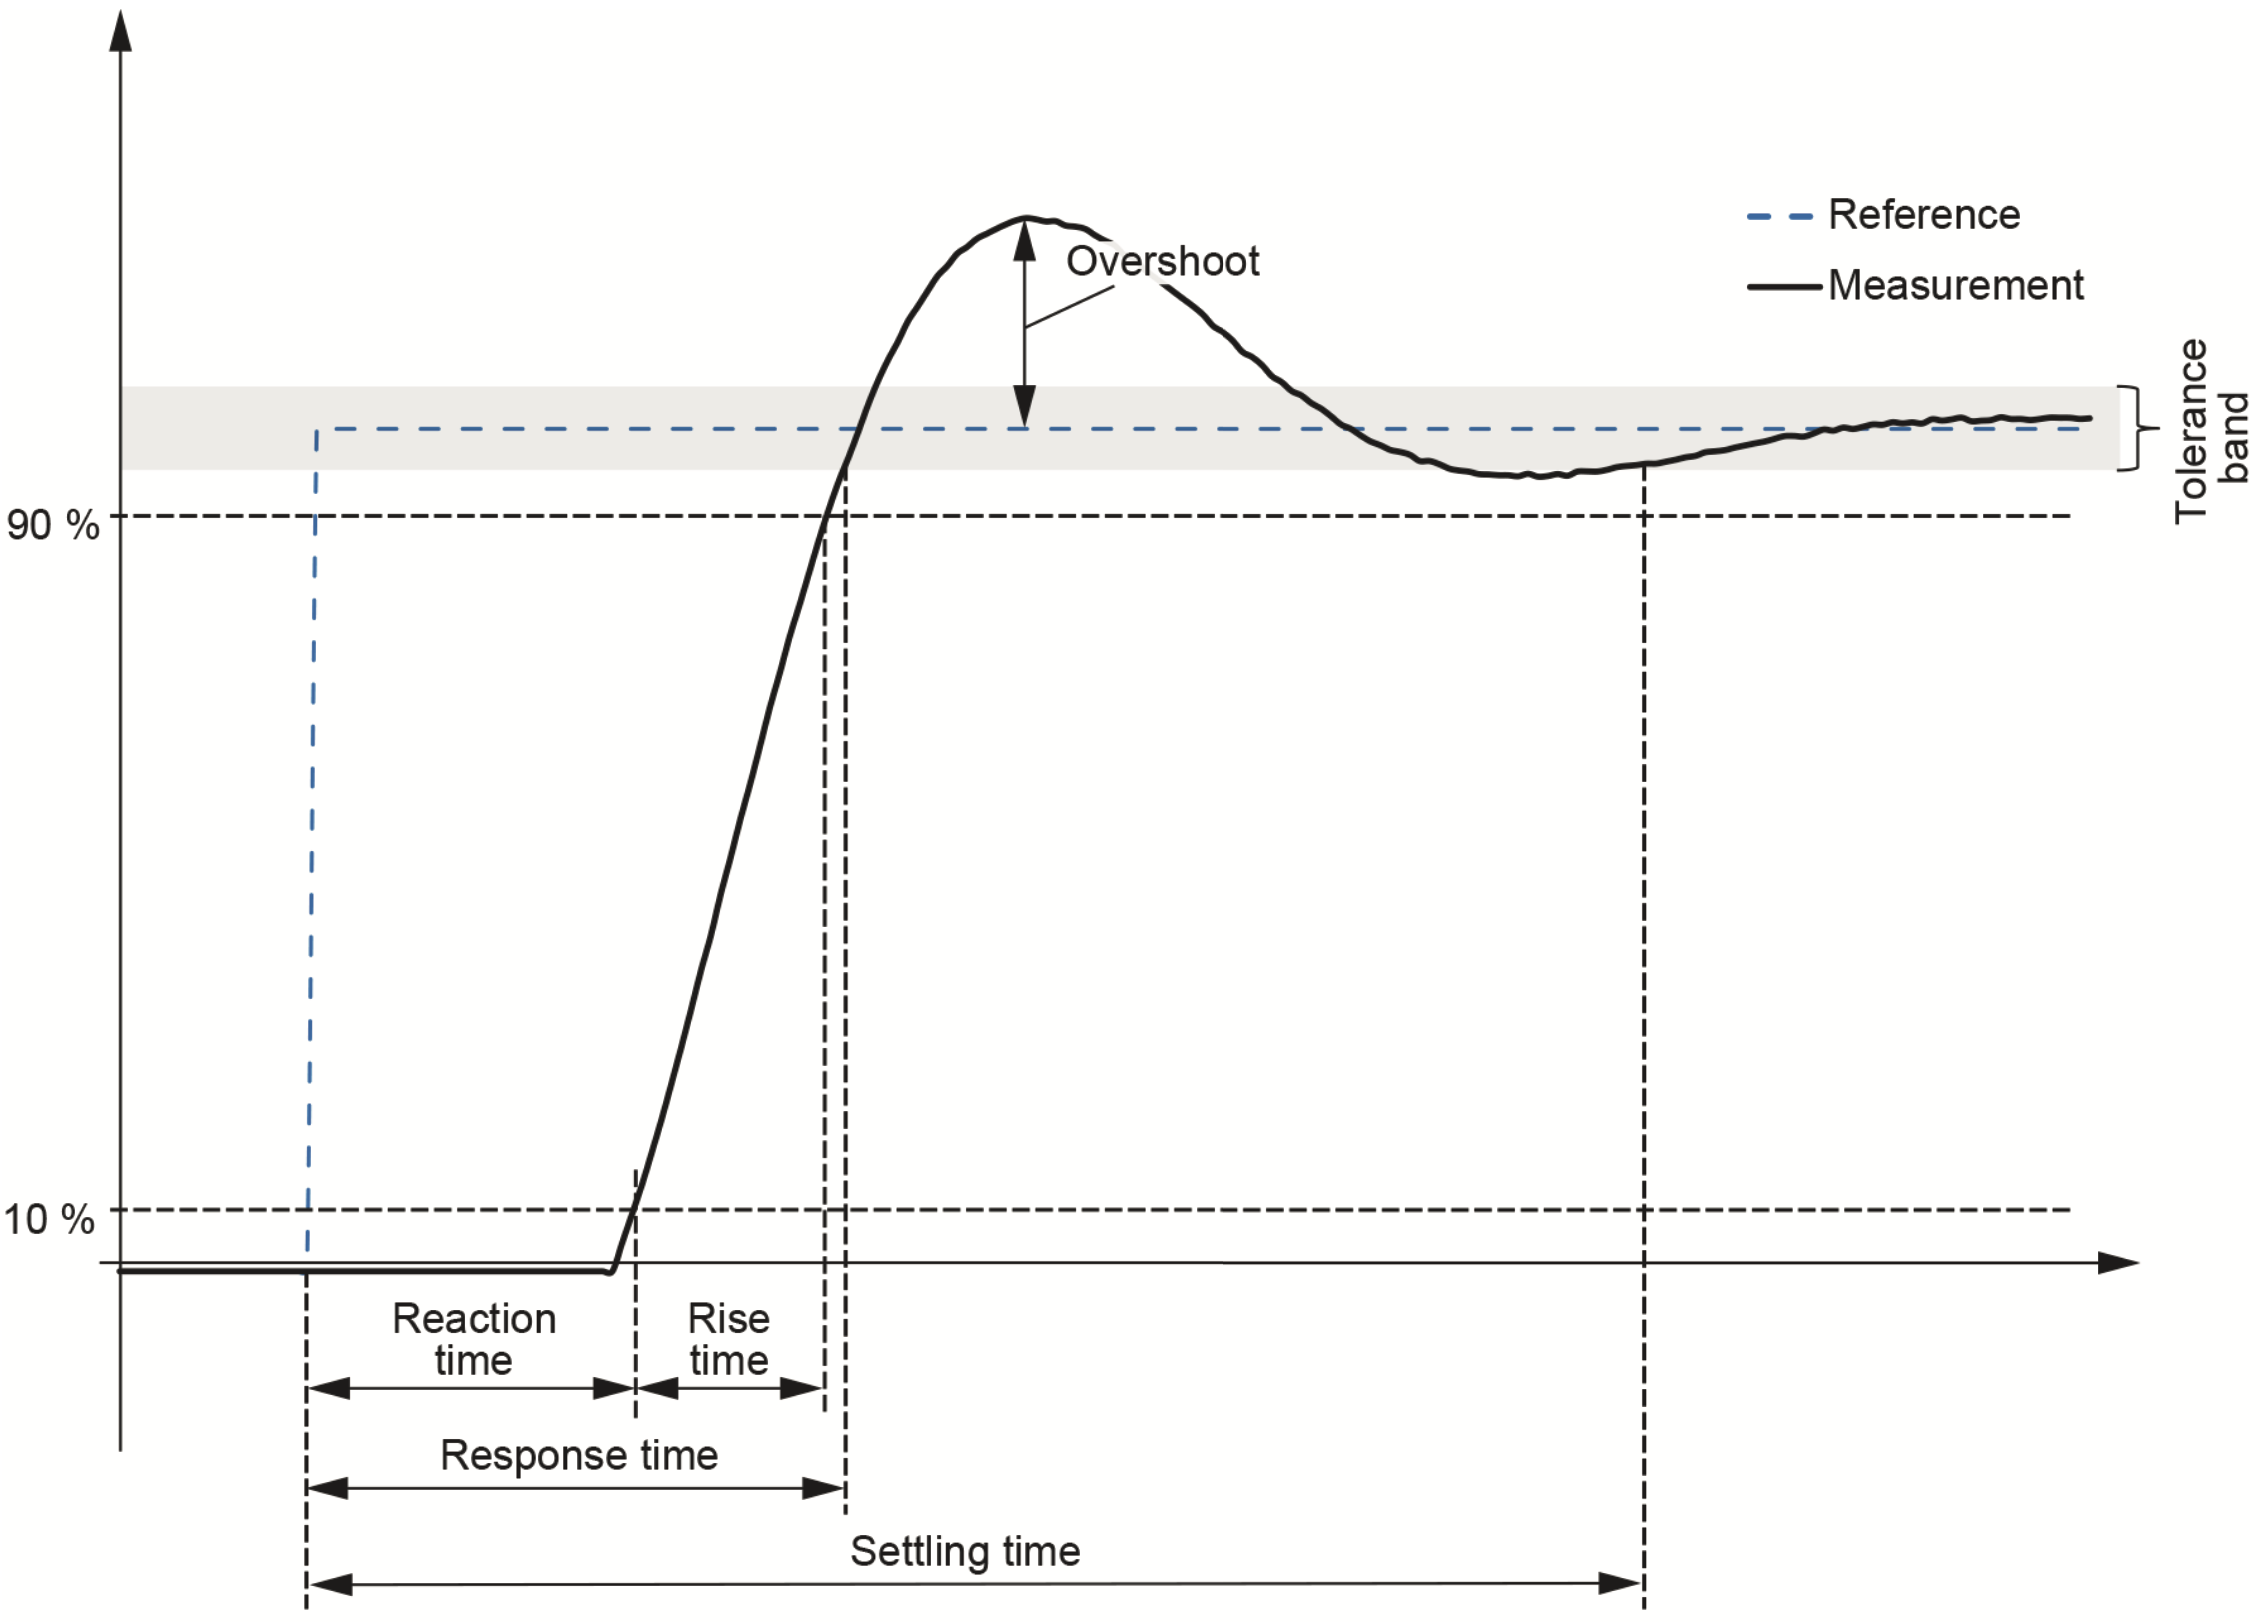
\includegraphics[width=\textwidth]{step_response_characteristics}

\end{document}
